\documentclass{oblivoir}
\usepackage{amsmath,amssymb,amsthm,kotex,mdframed,paralist,tabto,pifont}

\counterwithout{subsection}{section}
\newcounter{num}
\newcommand{\prob}[1]
{\bigskip\noindent\refstepcounter{num}\subsection{#1}}

\newcommand{\ans}{
{\par\medskip\begin{mdframed}
\textbf{풀이 : }
\vspace{0.6\textheight}
\end{mdframed}\par
\raggedleft\textbf{답 : (\qquad\qquad\qquad\qquad\qquad\qquad)}
\par}\bigskip\bigskip}

\newcommand\ov[2]{\ensuremath{\overline{#1#2}}}

\newcommand\ve[2]{\ensuremath{\overrightarrow{#1#2}}}

\newcommand{\pa}{\mathbin{\!/\mkern-5mu/\!}}

\TabPositions{0.2\textwidth,0.4\textwidth,0.6\textwidth,0.8\textwidth}
\newcommand\tabb[5]{\par\noindent
\ding{172}{#1}
\tab\ding{173}{#2}
\tab\ding{174}{#3}
\tab\ding{175}{#4}
\tab\ding{176}{#5}}

\newcounter{pnum}
\newcommand\pn{\stepcounter{pnum}\textbf{\thepnum}}

%%%
\begin{document}
\title{혜령 09 - 기하와 벡터[수능특강]\\
{\large 8단원 : 공간벡터}}
\author{}
\date{\today}
\maketitle
\tableofcontents

\newpage

%
\prob{08-예제2}
그림과 같이 한 모서리의 길이가 \(1\)인 정육면체 \(ABCD-EFGH\)의 꼭짓점을 시점과 종점으로 하고 크기가 \(\sqrt3\)인 벡터 중 서로 다른 벡터의 개수는?
(단, 영벡터는 제외한다.)
\begin{figure}[h!]
\centering
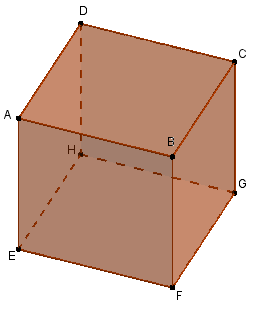
\includegraphics[width=0.4\textwidth]{01}
\end{figure}
\tabb{\(8\)}{\(12\)}{\(16\)}{\(20\)}{\(24\)}
\newpage

%
\prob{08-유제3}
그림과 같이 직육면체 \(ABCD-EFGH\)에서 삼각형 \(ACF\)의 무게중심을 \(P\)라고 하자.
\(\ve GP=l\ve AB+m\ve AD+n\ve AE\)를 만족시키는 세 실수 \(l\), \(m\), \(n\)에 대하여 \(l+m+n\)의 값은?
\begin{figure}[h!]
\centering
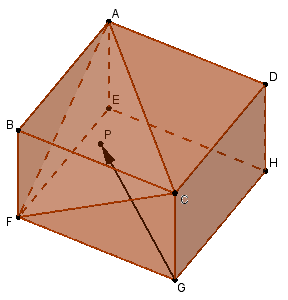
\includegraphics[width=0.4\textwidth]{02}
\end{figure}
\tabb{-\(\frac83\)}{-\(\frac73\)}{\(-2\)}{-\(\frac53\)}{-\(\frac43\)}

%
\prob{08-유제6}
좌표공간에 두 점 \(A(1,-2,a)\), \(B(3,1,2)\)가 있다.
원점 \(O\)에 대하여 \(\angle AOB=\frac\pi3\)일 때, \(a\)의 값은?
\tabb{\(-11\)}{\(-3\)}{\(0\)}{\(3\)}{\(11\)}

%
\prob{08-기초2}
좌표공간에 세 점 \(A(a,-3,5)\), \(B(3,b,2)\), \(C(5,3,-4)\)가 한 직선 위에 있을 때, \(\left|\ve AB\right|\)의 값은?
\tabb{\(\sqrt{10}\)}{\(\sqrt{11}\)}{\(2\sqrt3\)}{\(\sqrt{13}\)}{\(\sqrt{14}\)}
\newpage

%
\prob{08-기초3}
그림과 같이 모든 모서리의 길이가 \(4\)인 사각뿔 \(A-BCDE\)에서 두 모서리 \(AB\), \(AD\)의 중점을 각각 \(M\), \(N\)이라고 하자.
\(\ve CA\textbullet\left(\ve CM+\ve CN\right)\)의 값을 구하시오.
\begin{figure}[h!]
\centering
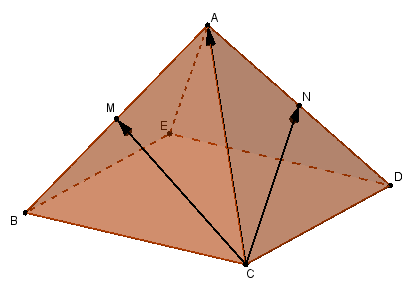
\includegraphics[width=0.7\textwidth]{03}
\end{figure}
\tabb{\(8\)}{\(12\)}{\(16\)}{\(20\)}{\(24\)}
\newpage

%
\prob{08-기본2}
사면체 \(ABC\)에서 \(\ov AD=\ov BD=\ov CD=2\)이고 \(\ov AD\perp\ov BD\), \(\ov BD\perp\ov CD\), \(\ov AD\perp\ov CD\)이다.
두 모서리 \(AB\), \(AC\)의 중점을 각각 \(E\), \(F\)라고 하고, 점 \(P\)가 모서리 \(BC\) 위의 점일 때, \(\left|\ve PE+\ve PF\right|\)의 최솟값은?
\begin{figure}[h!]
\centering
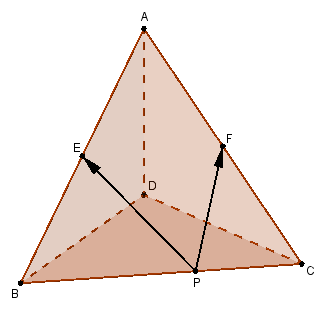
\includegraphics[width=0.5\textwidth]{04}
\end{figure}
\tabb{\(\sqrt3\)}{\(2\)}{\(\sqrt5\)}{\(\sqrt6\)}{\(\sqrt7\)}
\newpage

%
\prob{08-기본3}
그림은 한 변의 길이가 \(6\)인 정육각형을 밑변으로 하고 높이가 \(10\)인 육각기둥 \(ABCDEF-GHIJKL\)이다.
\(\ve GD\textbullet \ve HE\)의 값을 구하시오.
\begin{figure}[h!]
\centering
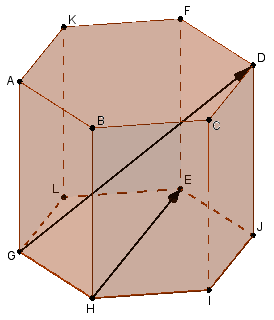
\includegraphics[width=0.55\textwidth]{05}
\end{figure}
\tabb{\(24\)}{\(36\)}{\(48\)}{\(60\)}{\(72\)}

\newpage

%
\prob{08-기본4}
그림과 같이 서로 수직인 두 선분 \(AB\), \(CD\)를 각각 두 밑면의 지름으로 하는 원뿔대가 있다.
\(\ov AB=2\), \(\ov CD=4\)이고, 선분 \(CD\)가 지름인 밑면에서 선분 \(CD\)와 수직인 지름의 양 끝점을 각각 \(E\), \(F\)라고 할 때, \(\ov AE=3\)이다.
두 벡터 \(\ve CA\), \ve DB가  이루는 각의 크기를 \(\theta\)라고 할 때, \(\cos\theta\)의 값은?
\begin{figure}[h!]
\centering
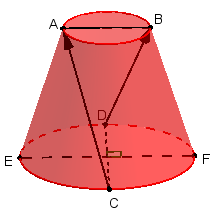
\includegraphics[width=0.4\textwidth]{06}
\end{figure}
\tabb{\(\frac13\)}{\(\frac3{10}\)}{\(\frac3{11}\)}{\(\frac14\)}{\(\frac3{13}\)}
\newpage

%
\prob{08-실력1}
좌표공간에서 두 구 \(S_1:x^2+y^2+z^2=20\), \(S_2:x^2+(y-6)^2+(z-8)^2=80\)의 중심을 각각 \(A\), \(B\)라고 하고, 두 구 \(S_1\), \(S_2\)가 만나서 생기는 원 \(C\) 위의 점 \(P\)에 대하여 \(\ve PA+\ve PB=\ve PQ\)를 만족시키는 점 \(Q\)가 나타내는 도형을 \(C'\)이라고 하자.
도형 \(C'\) 위를 움직이는 두 점 \(S\), \(T\)에 대하여 \(|\ve BS+\ve BT|\)의 최솟값을 구하여라.
\begin{figure}[h!]
\centering
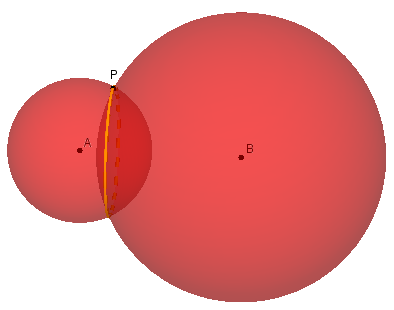
\includegraphics[width=0.8\textwidth]{07}
\end{figure}
\tabb{\(2\)}{\(4\)}{\(6\)}{\(8\)}{\(10\)}
\newpage

%
\prob{08-실력3}
그림과 같이 한 모서리의 길이가 \(2\)인 정육면체 \(ABCD-EFGH\)와 중심이 \(F\)이고 반지름의 길이가 \(2\)인 구가 있다.
두 모서리 \(AD\), \(GH\)의 중점을 각각 \(M\), \(N\)이라고 하고 두 선분 \(FM\), \(FN\)이 만나는 점을 각각 \(P\), \(Q\)라고 할 때, \(\ve PM\textbullet\ve FQ\)의 값은?
\begin{figure}[h!]
\centering
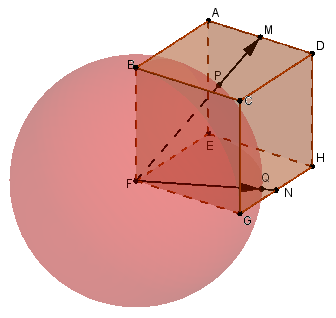
\includegraphics[width=0.6\textwidth]{08}
\end{figure}
\tabb{\(\frac8{15}\sqrt5\)}{\(\frac3{5}\sqrt5\)}{\(\frac2{3}\sqrt5\)}{\(\frac{11}{15}\sqrt5\)}{\(\frac4{5}\sqrt5\)}
\newpage

%%%%
\begin{table}[h!]
\begin{tabular}{|c|c||c|c||c|c||c|c|}
\hline
\pn&\ding{172}	&\pn&\ding{175}	&\pn&\ding{175}	&\pn&\ding{176}\\\hline
\pn&\ding{176}	&\pn&\ding{175}	&\pn&\ding{176}	&\pn&\ding{176}\\\hline
\pn&\ding{173}	&\pn&\ding{172}	&&				&&\\\hline
\end{tabular}
\end{table}

\end{document}